%============================================================================================================
%
%============================================================================================================

\documentclass[11pt, aspectratio=169]{beamer}
\usepackage{tikz}
\usetikzlibrary{calc, trees, positioning, arrows, chains, shapes.geometric, decorations.pathmorphing, shapes,  matrix, shapes.symbols}
\usepackage{caption, array, makecell, graphicx, booktabs, subfig, hyperref, amsmath, amssymb, amsfonts}
\captionsetup[figure]{labelformat=empty, font=footnotesize}
\usepackage[export]{adjustbox}
\usepackage[dvipsnames]{xcolor}


\hypersetup{
    colorlinks=true,
    linkcolor=RoyalBlue,
    citecolor=Green,
    filecolor=magenta,      
    urlcolor=RoyalBlue,
    pdftitle={Laboratory Studies of Cosmology-Inspired Defect Dynamics in Liquid Crystals},
    pdfauthor={Anik Mandal},
    bookmarksopen=true,
    bookmarksnumbered=true
}


\usetheme[sectionpage=none, numbering=fraction, progressbar=foot, block=fill, background=light ]{metropolis}
\useoutertheme{miniframes}
\setbeamerfont{footnote}{size=\scriptsize}
\addtobeamertemplate{footline}{\vspace{-1cm}}{}
\setbeamersize{text margin left=.5cm, text margin right=.5cm}


%=====| Adding custom thickness progress bar |===============================================================
\makeatletter
\setlength{\metropolis@progressinheadfoot@linewidth}{3pt} % Set thickness
\makeatother
\setbeamercolor{progress bar}{fg=red}

%=====| Adding section navigation bar at the top |===========================================================
\setbeamerfont{section in head/foot}{series=\bfseries}
\setbeamertemplate{headline}{%
  \begin{beamercolorbox}[wd=\paperwidth,ht=2ex,dp=1ex]{section in head/foot}
    \insertsectionnavigationhorizontal{\paperwidth}{}{}
  \end{beamercolorbox}
}

%=====| Adding custom reference in frames |==================================================================

\usepackage[backend=biber]{biblatex}
\addbibresource{references.bib}
\DeclareCiteCommand{\footcite}[\footnote]
  {\usebibmacro{prenote}}
  {%
    \printnames{labelname}%
    \space(\printfield{year})%
    \space
    \iffieldundef{doi}
      {%
        \printfield{journaltitle}%
        \setunit{\space}%
        \printfield{volume}%
        \setunit{\space}%
        \printfield{pages}%
      }
      {%
        \printfield{doi}%
      }%
  }
  {}
  {\usebibmacro{postnote}}


% \DeclareCiteCommand{\footcite}[\footnote]
%   {\usebibmacro{prenote}}
%   {\printnames{labelname}\space(\printfield{year})\space\printfield{doi}}
%   {}
%   {\usebibmacro{postnote}}



%=====| Adding custom Author–Date box in bottom-right corner |===============================================
\addtobeamertemplate{footline}{}{
  \begin{tikzpicture}[remember picture,overlay]
    \node[anchor=south east, xshift=-4pt, yshift=4pt] at (current page.south east) {
       \scalebox{0.9}{\textcolor{black!75}{\insertauthor; \insertdate}}
    };
  \end{tikzpicture}
}

% Title page informations ###################################################################################
\title{SLP Presentation}
\subtitle{Laboratory Studies of Cosmology-Inspired Defect Dynamics in Liquid Crystals}
\date{\today}
\author{Anik Mandal}
\institute{Ashoka University}
\titlegraphic{\hfill\includegraphics[height=1.75cm]{../tex-resource/ashoka-logo.png}}


\begin{document}

\maketitle
% \begin{frame}{Project objectives}
% \begin{itemize}
%     \item akjd
%     \item ajkdn
%     \item skdjn
% \end{itemize}
    
% \end{frame}

% \begin{frame}{Table of contents}
%   \setbeamertemplate{section in toc}[sections numbered]
%   \tableofcontents%[hideallsubsections]
% \end{frame}


\section[Intro]{Introduction}

\begin{frame}{Symmetry and Symmetry Breaking}

\begin{figure}
    \centering
    \subfloat[  $T > T_c$]{\includegraphics[width=0.3\linewidth, trim={0cm 0cm 0cm 0cm}, clip]{figs/imported/stable_ball.png}}\hspace{.1cm}
    \subfloat[$T < T_c$]{\includegraphics[width=0.3\linewidth, trim={0cm 0cm 0cm 0cm}, clip]{figs/imported/Unstable_ball.png}}\hspace{.1cm}
    \subfloat[Symmetry Breaking]{\includegraphics[width=0.3\linewidth]{figs//imported/Sym_breaking_ball.png}}
\end{figure}

\begin{itemize}
    \item[$\blacktriangleright$] Spontaneous symmetry breaking (SSB) ($T < T_c$) generates massive excitations via the Higgs mechanism.
    \item[$\blacktriangleright$] Early Universe evolution involves a hierarchy of symmetry-breaking events.\footcite{Kibble1982PhaseUniverse}$^,$\footcite{Vilenkin1985CosmicWalls}
\end{itemize}
\end{frame}


\begin{frame}{Formation of Topological Defects}
\begin{figure}
    \centering
    \subfloat[Domain Walls]{\includegraphics[width=0.3\linewidth]{figs/imported/domain_wall.png}}\hspace{.1cm}
    \subfloat[String Defects]{\includegraphics[width=0.3\linewidth]{figs/imported/string_defect.png}}
\end{figure}

\begin{itemize}
    \item[$\blacktriangleright$] Causally disconnected regions independently settle into different vacuum states, forming defects at the boundaries.\footcite{Kibble1976TopologyStrings}
    \item[$\blacktriangleright$] Cosmological defects acted as gravitational seeds for large-scale structure, drove CMB anisotropies, and remain viable candidates for dark matter.
\end{itemize}
    
\end{frame}


\begin{frame}[fragile]{Cosmology in the Laboratory}
\begin{itemize}
    \item[$\blacktriangleright$] In 1985, Zurek extended Kibble's idea to condensed matter physics. Where he tried to study the formation and dynamics of topological defects in quench-induced phase transitions in liquid $He$.\footcite{Zurek1985CosmologicalHelium}$^,$\footcite{Zurek1996CosmologicalSystems}
    \item[$\blacktriangleright$] Complexity of cryogenic experiments drove the adoption of liquid crystals as a robust alternative.\footcite{Chuang1991CosmologyCrystals}$^,$\footcite{Yurke1992CoarseningCrystals}$^,$\footcite{Fowler2017KibbleZurekCrystal}
\end{itemize}
\end{frame}

\begin{frame}{Kibble-Zurek Mechanism}
\begin{itemize}
    \item[$\blacktriangleright$] Critical slowing down causes the system to freeze out at time $\hat{t}$ when the relaxation time exceeds the quench rate $\tau_Q$, fixing a finite domain size $\hat{\xi}$ and leading to universal Kibble--Zurek scaling of defect density ($\rho$),
    \[
        \rho \propto \tau_Q^{-d\nu/(1+\nu z)},
    \]
    where $d$ is the effective defect dimension.
    
    \item[$\blacktriangleright$] After formation, defect networks coarsen to minimize the Frank elastic free energy, given in terms of the director field $\mathbf{n(r)}$ as,
    \[
        F=\frac{1}{2}\!\left[ K_1(\nabla\!\cdot\!\mathbf{n})^2 + K_2(\mathbf{n}\!\cdot\!\nabla\!\times\!\mathbf{n})^2 + K_3|\mathbf{n}\!\times\!\nabla\!\times\!\mathbf{n}|^2 \right],
    \]
    and in overdamped systems a one-scale model predicts universal late-time decay of defect density: $\rho(t)\!\propto\! t^{-1}$ (for  line defects) and $\rho(t)\!\propto\! t^{-1/2}$ (for domain walls).
\end{itemize}

\end{frame}


% Exp Setup==========================================================================================

\section{Experimental Setup}

\begin{frame}{Experimental Setup}
\begin{columns}

\begin{column}{0.2\textwidth}
\centering
\begin{tikzpicture}[
    node distance=0.25cm,
    every node/.style={draw, rectangle, rounded corners, minimum width=0.5cm, minimum height=0.5cm, text width=2.7cm, align=center},
    highlight/.style={draw=black, thick, fill=black!15, font=\footnotesize},
    faded/.style={draw=black!40, text=black, font=\scriptsize},
    arrow/.style={->, thick, draw=black!40}
]
\node[highlight] (1) {Patterning};
\node[highlight, below=of 1] (2) {Etching};
\node[highlight, below=of 2] (3) {Post etching treatment};
\node[highlight, below=of 3] (4) {Applying surfactant (DMOAP)};
\node[highlight, below=of 4] (5) {Cell assembly};
\node[highlight, below=of 5] (6) {Cell thickness measurement};
\node[highlight, below=of 6] (7) {LC filling and cooling};

\draw[arrow] (1) -- (2);
\draw[arrow] (2) -- (3);
\draw[arrow] (3) -- (4);
\draw[arrow] (4) -- (5);
\draw[arrow] (5) -- (6);
\draw[arrow] (6) -- (7);
\end{tikzpicture}
\end{column}

\begin{column}{0.8\textwidth}
\begin{figure}
    \centering
    \includegraphics[width=0.95\linewidth, trim = {0 0 0 2cm}, clip]{figs/imported/Fréedericksz_Transition.png}
    \caption{Fréedericksz transition due to electric field quench in\\ homeotropically aligned LC}
    \label{fig:placeholder}
\end{figure}
\end{column}

\end{columns}    
\end{frame}
% Patterning----------------------------------------------------------------------------------------
\begin{frame}{\small{Preparing Homeotropic Cell}}

\begin{columns}

\begin{column}{0.2\textwidth}

\centering  

\begin{tikzpicture}[
    node distance=0.25cm,
    every node/.style={draw, rectangle, rounded corners, minimum width=0.5cm, minimum height=0.5cm, text width=2.7cm, align=center},
    highlight/.style={draw=black, thick, fill=black!15},
    faded/.style={draw=black!40, text=black, font=\tiny},
    arrow/.style={->, thick, draw=black!40}
]
\node[highlight] (1) {Patterning};
\node[faded, below=0.5cm of 1] (2) {Etching};
\node[faded, below=of 2] (3) {Post etching treatment};
\node[faded, below=of 3] (4) {Applying surfactant (DMOAP)};
\node[faded, below=of 4] (5) {Cell assembly};
\node[faded, below=of 5] (6) {Cell thickness measurement};
\node[faded, below=of 6] (7) {LC filling and cooling};

\draw[arrow] (1) -- (2);
\draw[arrow] (2) -- (3);
\draw[arrow] (3) -- (4);
\draw[arrow] (4) -- (5);
\draw[arrow] (5) -- (6);
\draw[arrow] (6) -- (7);
\end{tikzpicture}

\end{column}

\begin{column}{0.8\textwidth}
\begin{itemize}
    \item[$\blacktriangleright$] ITO-coated glass cut to $4 \times 2\,\mathrm{cm}^2$.
    \item[$\blacktriangleright$] Conductive side identified using a multimeter.
    \item[$\blacktriangleright$] Cello tape masks $1\,\mathrm{cm}$ electrode region,
          leaving $0.5\,\mathrm{cm}$ gaps at both ends.
\end{itemize}
\begin{figure}
    \centering
    \includegraphics[width=0.5\linewidth, trim={0 8cm 0 10cm}, clip]{figs//imported/Cell_draw.png}
    \caption{Patterning}
    \label{fig:placeholder}
\end{figure}
\end{column}
\end{columns}

\end{frame}

% Eatching------------------------------------------------------------------------------------------
\begin{frame}{\small{Preparing Homeotropic Cell}}

\begin{columns}

\begin{column}{0.2\textwidth}

\centering
\begin{tikzpicture}[
    node distance=0.25cm,
    every node/.style={draw, rectangle, rounded corners, minimum width=0.5cm, minimum height=0.5cm, text width=2.7cm, align=center},
    highlight/.style={draw=black, thick, fill=black!15},
    faded/.style={draw=black!40, text=black, font=\tiny},
    arrow/.style={->, thick, draw=black!40}
]
\node[faded] (1) {Patterning};
\node[highlight, below=0.5cm of 1] (2) {Etching};
\node[faded, below=0.5cm of 2] (3) {Post etching treatment};
\node[faded, below=of 3] (4) {Applying surfactant (DMOAP)};
\node[faded, below=of 4] (5) {Cell assembly};
\node[faded, below=of 5] (6) {Cell thickness measurement};
\node[faded, below=of 6] (7) {LC filling and cooling};

\draw[arrow] (1) -- (2);
\draw[arrow] (2) -- (3);
\draw[arrow] (3) -- (4);
\draw[arrow] (4) -- (5);
\draw[arrow] (5) -- (6);
\draw[arrow] (6) -- (7);
\end{tikzpicture}

\end{column}

\begin{column}{0.8\textwidth}
\begin{itemize}
    \item[$\blacktriangleright$] Etching solution: concentrated HCl + Zn powder.
    \item[$\blacktriangleright$] Exposure time: 30 minutes (inside fume hood).
    \item[$\blacktriangleright$] Removes unprotected ITO, leaving defined electrodes.
    \item[$\blacktriangleright$] Rinsed with water and dilute base to neutralize acid.
\end{itemize}

\begin{figure}
    \centering
    \includegraphics[width=0.5\linewidth, trim={0 18cm 0 0}, clip]{figs//imported/Cell_draw.png}
    \caption{Eatching}
    \label{fig:placeholder}
\end{figure}

\end{column}
\end{columns}

\end{frame}

% Post etching--------------------------------------------------------------------------------------
\begin{frame}{\small{Preparing Homeotropic Cell}}

\begin{columns}

\begin{column}{0.2\textwidth}

\centering
\begin{tikzpicture}[
    node distance=0.25cm,
    every node/.style={draw, rectangle, rounded corners, minimum width=0.5cm, minimum height=0.5cm, text width=2.7cm, align=center},
    highlight/.style={draw=black, thick, fill=black!15},
    faded/.style={draw=black!40, text=black, font=\tiny},
    arrow/.style={->, thick, draw=black!40}
]
\node[faded] (1) {Patterning};
\node[faded, below=of 1] (2) {Etching};
\node[highlight, below=0.5cm of 2] (3) {Post etching treatment};
\node[faded, below=0.5cm of 3] (4) {Applying surfactant (DMOAP)};
\node[faded, below=of 4] (5) {Cell assembly};
\node[faded, below=of 5] (6) {Cell thickness measurement};
\node[faded, below=of 6] (7) {LC filling and cooling};

\draw[arrow] (1) -- (2);
\draw[arrow] (2) -- (3);
\draw[arrow] (3) -- (4);
\draw[arrow] (4) -- (5);
\draw[arrow] (5) -- (6);
\draw[arrow] (6) -- (7);
\end{tikzpicture}

\end{column}

\begin{column}{0.8\textwidth}
\begin{itemize}
    \item[$\blacktriangleright$] Etched glass cut into two symmetric electrode slabs.
    \item[$\blacktriangleright$] Manual scrubbing with soap and IPA removes loose residues.
    \item[$\blacktriangleright$] Ultrasonic cleaning: Soap-water bath for 15 minutes at 40-50$^\circ$C
    \item[$\blacktriangleright$] Final rinse with fresh IPA and dried using nitrogen gas to prevent streaking or residue.
\end{itemize}

\end{column}
\end{columns}

\end{frame}

% DMOAP---------------------------------------------------------------------------------------------
\begin{frame}{\small{Preparing Homeotropic Cell}}

\begin{columns}

\begin{column}{0.2\textwidth}

\centering
\begin{tikzpicture}[
    node distance=0.25cm,
    every node/.style={draw, rectangle, rounded corners, minimum width=0.5cm, minimum height=0.5cm, text width=2.7cm, align=center},
    highlight/.style={draw=black, thick, fill=black!15},
    faded/.style={draw=black!40, text=black, font=\tiny},
    arrow/.style={->, thick, draw=black!40}
]
\node[faded] (1) {Patterning};
\node[faded, below=of 1] (2) {Etching};
\node[faded, below=of 2] (3) {Post etching treatment};
\node[highlight, below=0.5cm of 3] (4) {Applying surfactant (DMOAP)};
\node[faded, below=0.5cm of 4] (5) {Cell assembly};
\node[faded, below=of 5] (6) {Cell thickness measurement};
\node[faded, below=of 6] (7) {LC filling and cooling};

\draw[arrow] (1) -- (2);
\draw[arrow] (2) -- (3);
\draw[arrow] (3) -- (4);
\draw[arrow] (4) -- (5);
\draw[arrow] (5) -- (6);
\draw[arrow] (6) -- (7);
\end{tikzpicture}

\end{column}

\begin{column}{0.8\textwidth}
\begin{itemize}
    \item[$\blacktriangleright$] 0.2\% DMOAP solution prepared in distilled water. Glass slabs dipped vertically for 5 minutes.
    \item[$\blacktriangleright$] Methoxy groups hydrolyze and bind to surface hydroxyl groups.
    \item[$\blacktriangleright$] Subsequent baking at 110$^\circ$C for 60 minutes.
    \item[$\blacktriangleright$] Forms strong covalent siloxane (Si-O-Si) bonds and molecules orient perpendicular to substrate.
\end{itemize}

\begin{figure}
    \centering
    \includegraphics[width=0.5\linewidth]{figs/imported/DMOAP.png}
    \caption{DMOAP structure}
    \label{fig:placeholder}
\end{figure}

\end{column}
\end{columns}

\end{frame}

% Cell assembly-------------------------------------------------------------------------------------
\begin{frame}{\small{Preparing Homeotropic Cell}}

\begin{columns}

\begin{column}{0.2\textwidth}

\centering
\begin{tikzpicture}[
    node distance=0.25cm,
    every node/.style={draw, rectangle, rounded corners, minimum width=0.5cm, minimum height=0.5cm, text width=2.7cm, align=center},
    highlight/.style={draw=black, thick, fill=black!15},
    faded/.style={draw=black!40, text=black, font=\tiny},
    arrow/.style={->, thick, draw=black!40}
]
\node[faded] (1) {Patterning};
\node[faded, below=of 1] (2) {Etching};
\node[faded, below=of 2] (3) {Post etching treatment};
\node[faded, below=of 3] (4) {Applying surfactant (DMOAP)};
\node[highlight, below=0.5cm of 4] (5) {Cell assembly};
\node[faded, below=0.5cm of 5] (6) {Cell thickness measurement};
\node[faded, below=of 6] (7) {LC filling and cooling};

\draw[arrow] (1) -- (2);
\draw[arrow] (2) -- (3);
\draw[arrow] (3) -- (4);
\draw[arrow] (4) -- (5);
\draw[arrow] (5) -- (6);
\draw[arrow] (6) -- (7);
\end{tikzpicture}

\end{column}

\begin{column}{0.5\textwidth}
\begin{itemize}
    \item[$\blacktriangleright$] DMOAP-treated slabs in sandwich geometry. 
    \item[$\blacktriangleright$] $23\,\mu\mathrm{m}$ Mylar film placed along the edges.
    \item[$\blacktriangleright$] Applied gentle pressure (30 min), then epoxy cured (24 h).
    \item[$\blacktriangleright$] Indium soldered to ITO electrodes.
\end{itemize}

\end{column}

\begin{column}{0.3\textwidth}
\begin{figure}
    \centering
    \includegraphics[width=\linewidth, trim={0 0 8cm 20cm}, clip]{figs//imported/Cell_draw.png}
    \caption{Cell assembly}
    \label{fig:placeholder}
\end{figure}
\end{column}

\end{columns}

\end{frame}

% Cell thickness------------------------------------------------------------------------------------
\begin{frame}{\small{Preparing Homeotropic Cell}}

\begin{columns}

\begin{column}{0.2\textwidth}

\centering
\begin{tikzpicture}[
    node distance=0.25cm,
    every node/.style={draw, rectangle, rounded corners, minimum width=0.5cm, minimum height=0.5cm, text width=2.7cm, align=center},
    highlight/.style={draw=black, thick, fill=black!15},
    faded/.style={draw=black!40, text=black, font=\tiny},
    arrow/.style={->, thick, draw=black!40}
]
\node[faded] (1) {Patterning};
\node[faded, below=of 1] (2) {Etching};
\node[faded, below=of 2] (3) {Post etching treatment};
\node[faded, below=of 3] (4) {Applying surfactant (DMOAP)};
\node[faded, below=of 4] (5) {Cell assembly};
\node[highlight, below=0.5cm of 5] (6) {Cell thickness measurement};
\node[faded, below=0.5cm of 6] (7) {LC filling and cooling};

\draw[arrow] (1) -- (2);
\draw[arrow] (2) -- (3);
\draw[arrow] (3) -- (4);
\draw[arrow] (4) -- (5);
\draw[arrow] (5) -- (6);
\draw[arrow] (6) -- (7);
\end{tikzpicture}

\end{column}

\begin{column}{0.4\textwidth}
\begin{itemize}
    \item[$\blacktriangleright$] Measured capacitance ($C$) via LCR meter; modeled as parallel plates to measured cell thickness as,
\end{itemize}
\[ d = \frac{\varepsilon_0 \varepsilon_r A}{C} \]
    
    \begin{itemize}
        \item[$\blacktriangleright$] Measured thickness: 
        \item 1st cell : $31.09 \pm 0.44\,\mu m$
        \item 2nd cell : $43.62 \pm 2.18\,\mu m$
    \end{itemize}
\end{column}

\begin{column}{0.4\textwidth}
\begin{figure}
    \centering
    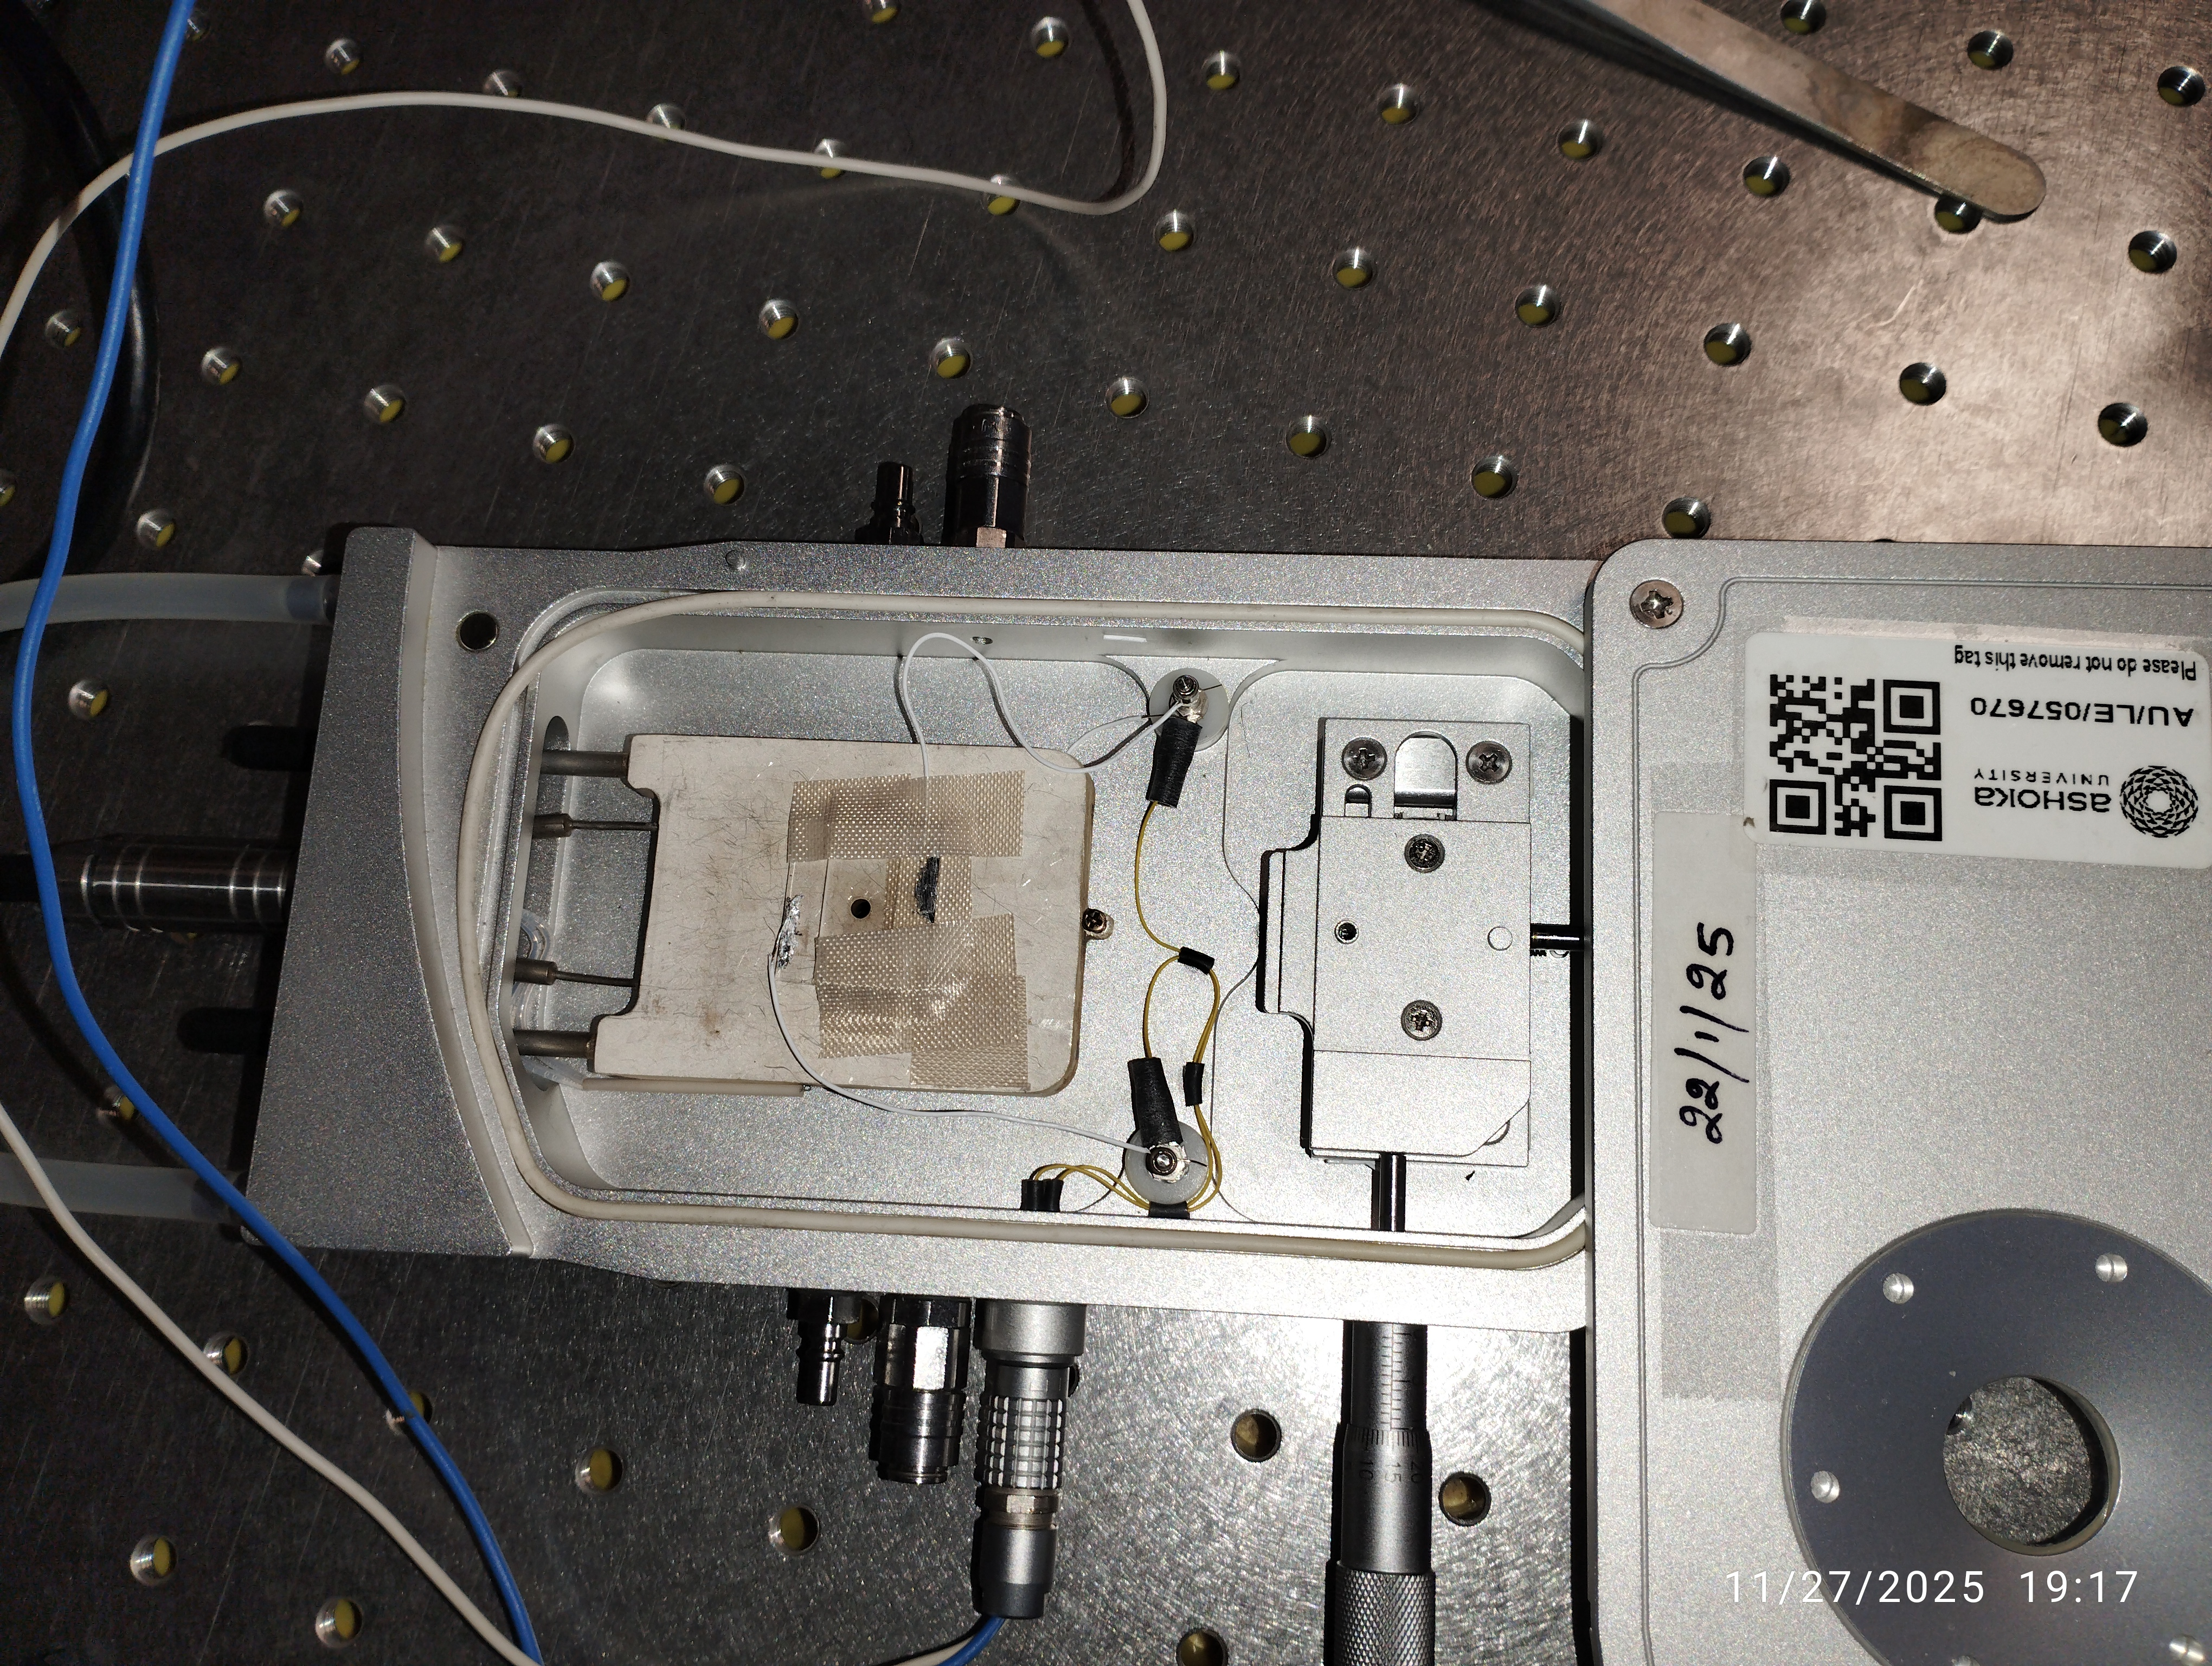
\includegraphics[width=\linewidth, trim={15cm 15cm 12cm 28cm}, clip]{figs//imported/Exp_LC_cell.jpg}
    \caption{Cell placed in a temperature-controlled \\ stage system}
    \label{fig:placeholder}
\end{figure}
\end{column}

\end{columns}
\end{frame}

% Cell thickness------------------------------------------------------------------------------------
\begin{frame}{\small{Preparing Homeotropic Cell}}

\begin{columns}

\begin{column}{0.2\textwidth}

\centering
\begin{tikzpicture}[
    node distance=0.25cm,
    every node/.style={draw, rectangle, rounded corners, minimum width=0.5cm, minimum height=0.5cm, text width=2.7cm, align=center},
    highlight/.style={draw=black, thick, fill=black!15},
    faded/.style={draw=black!40, text=black, font=\tiny},
    arrow/.style={->, thick, draw=black!40}
]
\node[faded] (1) {Patterning};
\node[faded, below=of 1] (2) {Etching};
\node[faded, below=of 2] (3) {Post etching treatment};
\node[faded, below=of 3] (4) {Applying surfactant (DMOAP)};
\node[faded, below=of 4] (5) {Cell assembly};
\node[faded, below=of 5] (6) {Cell thickness measurement};
\node[highlight, below=0.5cm of 6] (7) {LC filling and cooling};

\draw[arrow] (1) -- (2);
\draw[arrow] (2) -- (3);
\draw[arrow] (3) -- (4);
\draw[arrow] (4) -- (5);
\draw[arrow] (5) -- (6);
\draw[arrow] (6) -- (7);
\end{tikzpicture}

\end{column}

\begin{column}{0.5\textwidth}
\begin{block}{Thermal Protocol}
\begin{enumerate}
    \item Heat to 50$^\circ$C @ 20$^\circ$C/min, hold 10 min
    \item Cool to 36$^\circ$C @ 1$^\circ$C/min, hold 5 min
    \item Cool to 25$^\circ$C @ 0.1$^\circ$C/min
\end{enumerate}
\end{block}

\vspace{0.3cm}
\begin{itemize}
    \item[$\blacktriangleright$] MBBA introduced at elevated temperature.
    \item[$\blacktriangleright$] Capillary action fills the cell uniformly.
    \item[$\blacktriangleright$] Slow cooling minimizes defect formation.
\end{itemize}

\end{column}
\begin{column}{0.3\textwidth}
\begin{figure}
    \centering
    \includegraphics[width=\linewidth]{figs/imported/conoscopic_2_50X.png}
    \caption{Conoscopic image confirms\\ Homeotropic alignment}
    \label{fig:placeholder}
\end{figure}
    
\end{column}
\end{columns}

\end{frame}

% Final Setup------------------------------------------------------------------------------------
\begin{frame}{\small{Final Setup}}
\begin{itemize}
    \item[$\blacktriangleright$] 10-60 V RMS, 10 kHz Sine wave field has been generated using a \textit{ function generator} and \textit{A800DI Amplifier}. 
\end{itemize}
\begin{columns}
    \begin{column}{0.35\textwidth}
    \begin{itemize}
    \item[$\blacktriangleright$] Data taken at $28^\circ$C controlled temp; $10\times$ optical magnification.
    \end{itemize}
    \end{column}

    \begin{column}{0.65\textwidth}
        \begin{figure}
            \centering
            \subfloat{\includegraphics[width=0.35\linewidth]{figs//imported/Microscope.jpg}}\hspace{.1cm}
            \subfloat{\includegraphics[width=0.62\linewidth]{figs//imported/Exp_setup.jpg}}
            \caption{Experimental Setup}
            \label{fig:placeholder}
        \end{figure}
    \end{column}
    
\end{columns}
\end{frame}

% Comp Setup==========================================================================================
\section{Computational Framework}

\begin{frame}{Computational Framework\footnote{Clone: \$ git clone https://github.com/mandal-anik10/SLP-CosmoWithLCs.git}}
\begin{columns}


\begin{column}{0.2\textwidth}
\centering
\begin{tikzpicture}[
    node distance=0.25cm,
    every node/.style={draw, rectangle, rounded corners, minimum width=0.5cm, minimum height=0.5cm, text width=2.7cm, align=center},
    highlight/.style={draw=black, thick, fill=black!15, font=\footnotesize},
    faded/.style={draw=black!40, text=black, font=\tiny},
    arrow/.style={->, thick, draw=black!40}
]
\node[highlight] (1) {Pre-processing and noise reduction};
\node[highlight, below=of 1] (2) {Ridge detection};
\node[highlight, below=of 2] (3) {Hysteresis thresholding};
\node[highlight, below=of 3] (4) {Binary closing and cleaning};
\node[highlight, below=of 4] (5) {Skeletonizing};
\node[highlight, below=of 5] (6) {Estimating defect density};

\draw[arrow] (1) -- (2);
\draw[arrow] (2) -- (3);
\draw[arrow] (3) -- (4);
\draw[arrow] (4) -- (5);
\draw[arrow] (5) -- (6);

\end{tikzpicture}
\end{column}

\begin{column}{0.8\textwidth}
$\blacktriangleright$ Developed an automated image processing pipeline to quantify defect density frame-by-frame.
\end{column}

\end{columns}
\end{frame}

% Noise reduction-----------------------------------------------------------------------------------
\begin{frame}{Computational Framework}
\begin{columns}

\begin{column}{0.2\textwidth}
\centering
\begin{tikzpicture}[
    node distance=0.25cm,
    every node/.style={draw, rectangle, rounded corners, minimum width=0.5cm, minimum height=0.5cm, text width=2.7cm, align=center},
    highlight/.style={draw=black, thick, fill=black!15},
    faded/.style={draw=black!40, text=black, font=\tiny},
    arrow/.style={->, thick, draw=black!40}
]
\node[highlight] (1) {Pre-processing and noise reduction};
\node[faded, below=0.5cm of 1] (2) {Ridge detection};
\node[faded, below=of 2] (3) {Hysteresis thresholding};
\node[faded, below=of 3] (4) {Binary closing and cleaning};
\node[faded, below=of 4] (5) {Skeletonizing};
\node[faded, below=of 5] (6) {Estimating defect density};

\draw[arrow] (1) -- (2);
\draw[arrow] (2) -- (3);
\draw[arrow] (3) -- (4);
\draw[arrow] (4) -- (5);
\draw[arrow] (5) -- (6);

\end{tikzpicture}
\end{column}

\begin{column}{0.8\textwidth}
    \begin{itemize}
        \item[$\blacktriangleright$] $3\times3$-median filter suppresses impulsive noise by replacing each pixel value with the median of its $3\times3$ neighborhood.
        \item[$\blacktriangleright$] Preserves sharp edges and fine structural details better than linear filters.
    \end{itemize}
\vspace{\fill}
\begin{figure}[]
    \centering
    \includegraphics[width=\linewidth, trim={0cm 1.75cm 0cm 1.75cm}, clip]{figs/test-framework-1_50s_28_60V_5-S012.png}
    \caption{\footnotesize{(L) Original, (C) Denoised, (R) Ridge Map}}
    \label{fig:CF_Noise}
\end{figure}
\end{column}

\end{columns}
\end{frame}

% Ridge detection-----------------------------------------------------------------------------------
\begin{frame}{Computational Framework}
\begin{columns}

\begin{column}{0.2\textwidth}
\centering
\begin{tikzpicture}[
    node distance=0.25cm,
    every node/.style={draw, rectangle, rounded corners, minimum width=0.5cm, minimum height=0.5cm, text width=2.7cm, align=center},
    highlight/.style={draw=black, thick, fill=black!15},
    faded/.style={draw=black!40, text=black, font=\tiny},
    arrow/.style={->, thick, draw=black!40}
]
\node[faded] (1) {Pre-processing and noise reduction};
\node[highlight, below=0.5cm of 1] (2) {Ridge\\ detection};
\node[faded, below=0.5cm of 2] (3) {Hysteresis thresholding};
\node[faded, below=of 3] (4) {Binary closing and cleaning};
\node[faded, below=of 4] (5) {Skeletonizing};
\node[faded, below=of 5] (6) {Estimating defect density};

\draw[arrow] (1) -- (2);
\draw[arrow] (2) -- (3);
\draw[arrow] (3) -- (4);
\draw[arrow] (4) -- (5);
\draw[arrow] (5) -- (6);

\end{tikzpicture}
\end{column}

\begin{column}{0.8\textwidth}
    \begin{itemize}
        \item[$\blacktriangleright$] Applied modified Hessian-based Meijering\footcite{Meijering2004DesignImages} ridge detection filter.
        \item[$\blacktriangleright$] A modified Hessian matrix was constructed as
        \[
        H_f'(x)=
        \begin{bmatrix}
        f_{xx}+\alpha f_{yy} & (1-\alpha)f_{xy} \\
        (1-\alpha)f_{xy} & f_{yy}+\alpha f_{xx}
        \end{bmatrix}.
        \] Where $f_{ij}(x,y) = (f*\frac{\partial^2G}{\partial_i\partial_j})(x,y)$, for the image $f$ and normalized Gaussian kernel $G$, $\alpha=1/3$ for 2D image.
        \item[$\blacktriangleright$] Eigenvalues of $H_f'(x)$ were used to compute a ``neuriteness" measure per pixel.
        \item[$\blacktriangleright$] The eigenvector corresponding to the smaller absolute eigenvalue($\geq 0$) defines the local ridge direction.
    
    \end{itemize}
\end{column}

\end{columns}
\end{frame}

% Hysteresis thresholding---------------------------------------------------------------------------
\begin{frame}{Computational Framework}
\begin{columns}

\begin{column}{0.2\textwidth}
\centering
\begin{tikzpicture}[
    node distance=0.25cm,
    every node/.style={draw, rectangle, rounded corners, minimum width=0.5cm, minimum height=0.5cm, text width=2.7cm, align=center},
    highlight/.style={draw=black, thick, fill=black!15},
    faded/.style={draw=black!40, text=black, font=\tiny},
    arrow/.style={->, thick, draw=black!40}
]
\node[faded] (1) {Pre-processing and noise reduction};
\node[faded, below=of 1] (2) {Ridge detection};
\node[highlight, below=0.5cm of 2] (3) {Hysteresis thresholding};
\node[faded, below=0.5cm of 3] (4) {Binary closing and cleaning};
\node[faded, below=of 4] (5) {Skeletonizing};
\node[faded, below=of 5] (6) {Estimating defect density};

\draw[arrow] (1) -- (2);
\draw[arrow] (2) -- (3);
\draw[arrow] (3) -- (4);
\draw[arrow] (4) -- (5);
\draw[arrow] (5) -- (6);

\end{tikzpicture}
\end{column}

\begin{column}{0.8\textwidth}
\begin{itemize}
    \item[$\blacktriangleright$] Applied hysteresis thresholds to suppress spurious ridges.
    \item[$\blacktriangleright$] Retained pixels $> Th_{\text{high}}$, and those $> Th_{\text{low}}$ only if connected to already-classified defect pixels through 8-connectivity neighborhoods.
\end{itemize}
\vspace{\fill}
\begin{figure}[b]
    \centering
    \includegraphics[width=\linewidth, trim={0cm 1.75cm 0cm 1.75cm}, clip]{figs/test-framework-1_50s_28_60V_5-S345.png}
    \caption{\footnotesize{ (L)Hysteresis threshold, (C)cleaned, (R) Skeletonized}}
    \label{fig:CF_HystTh}
\end{figure}
\end{column}

\end{columns}
\end{frame}

% Binary closing and cleaning-----------------------------------------------------------------------
\begin{frame}{Computational Framework}
\begin{columns}

\begin{column}{0.2\textwidth}
\centering
\begin{tikzpicture}[
    node distance=0.25cm,
    every node/.style={draw, rectangle, rounded corners, minimum width=0.5cm, minimum height=0.5cm, text width=2.7cm, align=center},
    highlight/.style={draw=black, thick, fill=black!15},
    faded/.style={draw=black!40, text=black, font=\tiny},
    arrow/.style={->, thick, draw=black!40}
]
\node[faded] (1) {Pre-processing and noise reduction};
\node[faded, below=of 1] (2) {Ridge detection};
\node[faded, below=of 2] (3) {Hysteresis thresholding};
\node[highlight, below=0.5cm of 3] (4) {Binary closing and cleaning};
\node[faded, below=0.5cm of 4] (5) {Skeletonizing};
\node[faded, below=of 5] (6) {Estimating defect density};

\draw[arrow] (1) -- (2);
\draw[arrow] (2) -- (3);
\draw[arrow] (3) -- (4);
\draw[arrow] (4) -- (5);
\draw[arrow] (5) -- (6);

\end{tikzpicture}
\end{column}

\begin{column}{0.8\textwidth}
\begin{itemize}
    \item[$\blacktriangleright$] Applied binary closing to fill gaps and ensure defect line continuity. 
    \item[$\blacktriangleright$] Eliminated isolated noise and fragments via a minimum length threshold.
\end{itemize}
\vspace{\fill}
\begin{figure}[b]
    \centering
    \includegraphics[width=\linewidth, trim={0cm 1.75cm 0cm 1.75cm}, clip]{figs/test-framework-1_50s_28_60V_5-S345.png}
    \caption{\footnotesize{ (L)Hysteresis threshold, (C)cleaned, (R) Skeletonized}}
    \label{fig:CF_BinaryClosing}
\end{figure}
\end{column}

\end{columns}
\end{frame}

% Skletonizing--------------------------------------------------------------------------------------
\begin{frame}{Computational Framework}
\begin{columns}

\begin{column}{0.2\textwidth}
\centering
\begin{tikzpicture}[
    node distance=0.25cm,
    every node/.style={draw, rectangle, rounded corners, minimum width=0.5cm, minimum height=0.5cm, text width=2.7cm, align=center},
    highlight/.style={draw=black, thick, fill=black!15},
    faded/.style={draw=black!40, text=black, font=\tiny},
    arrow/.style={->, thick, draw=black!40}
]
\node[faded] (1) {Pre-processing and noise reduction};
\node[faded, below=of 1] (2) {Ridge detection};
\node[faded, below=of 2] (3) {Hysteresis thresholding};
\node[faded, below=of 3] (4) {Binary closing and cleaning};
\node[highlight, below=0.5cm of 4] (5) {Skeletonizing};
\node[faded, below=0.5cm of 5] (6) {Estimating defect density};

\draw[arrow] (1) -- (2);
\draw[arrow] (2) -- (3);
\draw[arrow] (3) -- (4);
\draw[arrow] (4) -- (5);
\draw[arrow] (5) -- (6);

\end{tikzpicture}
\end{column}

\begin{column}{0.8\textwidth}
\begin{itemize}
    \item[$\blacktriangleright$] Applied morphological thinning to collapse wide defect regions into their fundamental medial axis.
    \item[$\blacktriangleright$] Preserves the object's topology and connectivity, ensuring the skeleton represents the original structure.
\end{itemize}
\vspace{\fill}
\begin{figure}[b]
    \centering
    \includegraphics[width=\linewidth, trim={0cm 1.75cm 0cm 1.75cm}, clip]{figs/test-framework-1_50s_28_60V_5-S345.png}
    \caption{\footnotesize{ (L)Hysteresis threshold, (C)cleaned, (R) Skeletonized}}
    \label{fig:CF_BinaryClosing}
\end{figure}
\end{column}

\end{columns}
\end{frame}

% Defect density------------------------------------------------------------------------------------
\begin{frame}{Computational Framework}
\begin{columns}

\begin{column}{0.2\textwidth}
\centering
\begin{tikzpicture}[
    node distance=0.25cm,
    every node/.style={draw, rectangle, rounded corners, minimum width=0.5cm, minimum height=0.5cm, text width=2.7cm, align=center},
    highlight/.style={draw=black, thick, fill=black!15},
    faded/.style={draw=black!40, text=black, font=\tiny},
    arrow/.style={->, thick, draw=black!40}
]
\node[faded] (1) {Pre-processing and noise reduction};
\node[faded, below=of 1] (2) {Ridge detection};
\node[faded, below=of 2] (3) {Hysteresis thresholding};
\node[faded, below=of 3] (4) {Binary closing and cleaning};
\node[faded, below=of 4] (5) {Skeletonizing};
\node[highlight, below=0.5cm of 5] (6) {Estimating defect density};

\draw[arrow] (1) -- (2);
\draw[arrow] (2) -- (3);
\draw[arrow] (3) -- (4);
\draw[arrow] (4) -- (5);
\draw[arrow] (5) -- (6);

\end{tikzpicture}
\end{column}

\begin{column}{0.8\textwidth}
\begin{itemize}
    \item[$\blacktriangleright$] Utilized the \textit{Skan} library to model the skeleton as a network graph, summing branch lengths based on pixel connectivity.
    \item[$\blacktriangleright$] Total defect length computed by summing the lengths of all skeleton branches.
    \item[$\blacktriangleright$] Defect density derived by dividing the total length by the sample volume ($V$), given by $\rho = L / V$.
\end{itemize}
\end{column}

\end{columns}
\end{frame}

\begin{frame}{Error Analysis: Temporal Uncertainty}
\begin{itemize}
    \item $\sim30\%$ frame drop at 100 fps (write-speed limit) caused non-uniform temporal distortion.
    \item Reconstruct a statistically true timeline using Monte Carlo resampling.
\end{itemize}

\begin{block}{Monte Carlo Time Correction}
    \begin{itemize}
        \item Resampled frame sequence 1000 times with $100/70$ time rescaling to account for the frame drops.
        \item Defined corrected timestamp as:
        \[ t_i = \mu_{t_i} \pm \sigma_{t_i} \]
        \item Median $\mu_{t_i}$ used as true time of the frames; $\sigma_{t_i}$ tracks uncertainty\footnote{Horizontal error bars omitted from the plots for visual clarity}.
    \end{itemize}
\end{block}

\end{frame}

\begin{frame}{Error Analysis: Systematic Error in Defect Density}
1. Error in area measurement ($5\%$)
    \begin{itemize}
        \item Error of $2\,\mathrm{mm}$ in unit length $\Rightarrow$ $4\,\mathrm{mm}^2$ error in area ($A=80\,\mathrm{mm}^2$).
        \item Propagates linearly to density: \[ \frac{d\rho}{\rho} \approx \frac{dA}{A} \approx 5\% \]
    \end{itemize} 

2.  Error in  calibration scale ($0.3\%$)
    \begin{itemize}
        \item Scale bar ($1174\,\mathrm{px}$) has edge width ($1\sigma$) uncertainty of $3.6\,\mathrm{px}$.
        \item Propagates inversely ($\rho \propto C^{-1}$): \[ \frac{d\rho}{\rho} \approx \frac{dC}{C} = \frac{3.6}{1174} \approx 0.3\% \]
    \end{itemize}

\centering
\textbf{Total Systematic Uncertainty: $5.3\%$}
\end{frame}

\begin{frame}{Error Analysis: Stochastic error in defect density}
\begin{columns}

\begin{column}{0.4\textwidth}
    $\blacktriangleright$ Quantified stochastic error via mean ($\bar{x}$) and standard deviation($\sigma$) of independent trials ($N=5$, for defect formation $N=3$).
\[
    x = \bar{x} \pm \sigma = \frac{1}{N}\sum_{i=1}^{N} x_i \pm \sqrt{\frac{\sum_{i=1}^{N}(x_i - \bar{x})^2}{N-1}}
\]\\
$\blacktriangleright$ \textbf{Relative error selection criteria:}
20-point median of relative errors\\
\[
median \left( \frac{\sigma}{\bar{x}}(t)\right) < 0.1
\] 

\end{column}

\begin{column}{0.6\textwidth}
    \begin{figure}
    \centering
    \includegraphics[width=\linewidth, trim={1cm 0.5cm 2.5cm 2cm}, clip]{figs/datapoint_selection_criteria.png}
    \caption{\footnotesize{This example figure (60V data) shows the region selected based on the selection criteria.}}
    \label{fig:placeholder}
\end{figure}
\end{column}

\end{columns}    
\end{frame}

%uytfkuyvhj

\section{Defect Dynamics}
\begin{frame}{Late time dynamics: cell with permanent defects}
\begin{columns}
    \begin{column}{0.55\textwidth}
    \begin{figure}
    \centering
    \includegraphics[width=\linewidth, trim={0.5cm 0.5cm 0.5cm 0.5cm}, clip]{figs/imported/pi_wall.png}
    \caption{\footnotesize{(Left) Observed under a cross polarizer, a pair of $\pm1/2$ wedge disclinations connected by a $\pi$-wall when an in-plane electric field is present. (Right) Sketch of the 2D director field; $\theta$ is the angle between the $\pi$-wall and the electric field. (Source\footcite{Blanc2005DynamicsBackflow})}}
    \label{fig:placeholder}
    \end{figure}
    \end{column}

    \begin{column}{0.45\textwidth}
    \begin{figure}
    \centering
    \includegraphics[width=\linewidth, trim={0.5cm 0.5cm 0.5cm 0.5cm}, clip]{figs/old_60V_dyn.png}
    \caption{\footnotesize{Topological defects at different time stamps for 60V at 10$\times$ resolution.}}
    \label{fig:placeholder}
    \end{figure}
        
    \end{column}
\end{columns}
\end{frame}

\begin{frame}{Late time dynamics: cell with permanent defects}
    \begin{figure}[h]
    \centering
    \subfloat[10V : -1.20]{\includegraphics[width=0.5\textwidth, trim={1.5cm 0.5cm 3cm 1.5cm}, clip]{figs/10V-rho_dyn.png}}
    \subfloat[20V : -0.80]{\includegraphics[width=0.5\textwidth, trim={1.5cm 0.5cm 3cm 1.5cm}, clip]{figs/20V-rho_dyn.png}}
    % \caption{\footnotesize{late-time coarsening dynamics of defect density ($\rho$) versus time ($t$) for the 10V, 20V, 40V, 60V applied field case, observed at $10\times$ magnification.}}
    \label{fig:old_dyn_string_density}
    \end{figure}
\end{frame}

\begin{frame}{Late time dynamics: cell with permanent defects}
    \begin{figure}[h]
    \centering
    \subfloat[40V : -0.98]{\includegraphics[width=0.5\textwidth, trim={1.5cm 0.5cm 3cm 1.5cm}, clip]{figs/40V-rho_dyn.png}}
    \subfloat[60V : -1.02]{\includegraphics[width=0.5\textwidth, trim={1.5cm 0.5cm 3cm 1.5cm}, clip]{figs/60V-rho_dyn.png}}
    % \caption{\footnotesize{late-time coarsening dynamics of defect density ($\rho$) versus time ($t$) for the 10V, 20V, 40V, 60V applied field case, observed at $10\times$ magnification.}}
    \label{fig:old_dyn_string_density}
    \end{figure}
\end{frame}

\begin{frame}{Late time dynamics: cell without permanent defects}
\begin{columns}
    \begin{column}{0.6\textwidth}
    \begin{figure}
    \centering
    \includegraphics[width=\linewidth, trim={0.5cm 0.5cm 0.5cm 0.5cm}, clip]{figs/imported/domain_dyn.png}
    \caption{\footnotesize{(Left) Observed under a cross polarizer, a pair of $\pm1/2$ wedge disclinations connected by a $\pi$-wall when an in-plane electric field is present. (Right) Sketch of the 2D director field; $\theta$ is the angle between the $\pi$-wall and the electric field. (Source\footcite{Blanc2005DynamicsBackflow})}}
    \label{fig:placeholder}
    \end{figure}
    \end{column}

    \begin{column}{0.4\textwidth}
    \begin{figure}
    \centering
    \includegraphics[width=\linewidth, trim={0.5cm 0.5cm 0.5cm 0.5cm}, clip]{figs/28_new_60V_dyn.png}
    \caption{\footnotesize{Topological defects at different time stamps for 60V at 10$\times$ resolution.}}
    \label{fig:placeholder}
    \end{figure}
        
    \end{column}
\end{columns}
    
\end{frame}

\begin{frame}{Late time dynamics: cell without permanent defects}
    \begin{figure}[h]
    \centering
    \subfloat[10V : -0.74]{\includegraphics[width=0.5\textwidth, trim={1cm 0 2cm 1cm}, clip]{figs/28_new_10V_scalling.png}}
    \subfloat[20V : -0.21]{\includegraphics[width=0.5\textwidth, trim={1cm 0 2cm 1cm}, clip]{figs/28_new_20V_scalling.png}}
    % \caption{ \textbf{New cell without permanent defects}: Log-log plot showing the late-time coarsening dynamics of defect density ($\rho$) versus time ($t$) for the 10V, 20V, 40V, 60V applied field case, observed at $10\times$ magnification. The solid blue line represents the average of the estimated defect length, with the surrounding shaded region indicating the $1\sigma$ limits of random error. The orange line depicts the best power-law fit within the scaling regime. The shaded red regions mark data excluded from the analysis: early-time data (left) were discarded to remove the initial 10–25 frames, while the late-time tail (right) was excluded based on relative error selection criteria.}
    \label{fig:dyn_string_density}
    \end{figure}
    
\end{frame}

\begin{frame}{Late time dynamics: cell without permanent defects}

    \begin{figure}[h]
    \centering
    \subfloat[40V : -0.22]{\includegraphics[width=0.5\textwidth, trim={1cm 0 2cm 1cm}, clip]{figs/28_new_40V_scalling.png}}
    \subfloat[60V : -0.33]{\includegraphics[width=0.5\textwidth, trim={1cm 0 2cm 1cm}, clip]{figs/28_new_60V_scalling.png}}
    % \caption{ \textbf{New cell without permanent defects}: Log-log plot showing the late-time coarsening dynamics of defect density ($\rho$) versus time ($t$) for the 10V, 20V, 40V, 60V applied field case, observed at $10\times$ magnification. The solid blue line represents the average of the estimated defect length, with the surrounding shaded region indicating the $1\sigma$ limits of random error. The orange line depicts the best power-law fit within the scaling regime. The shaded red regions mark data excluded from the analysis: early-time data (left) were discarded to remove the initial 10–25 frames, while the late-time tail (right) was excluded based on relative error selection criteria.}
    \label{fig:dyn_string_density}
    \end{figure}
\end{frame}

\begin{frame}{Formation dynamics}
\begin{columns}

\begin{column}{0.7\textwidth}
\begin{figure}
    \centering
    \includegraphics[width=\linewidth]{figs/formation_dyn.png}
    \caption{Observed freeze-out of director dynamics and strong stochasticity at high electric field frequency(10Hz)}
    \label{fig:formation_dyn}
\end{figure}
\end{column}

\begin{column}{0.3\textwidth}
    \begin{figure}
        \centering
        \includegraphics[width=\linewidth]{figs/electro_convection_2025-12-01T20-15-08.641.png}
        \caption{Electroconvection observed in the prepared MBBA LC at electric field frequency $\sim Hz$ }
        \label{fig:placeholder}
    \end{figure}
\end{column}
    
\end{columns}
\end{frame}


\section{Conclusion}
\begin{frame}[fragile]{Conclusion}
    \begin{itemize}
        \item[$\blacktriangleright$] \textbf{Late-Time Dynamics}
        \begin{itemize}
            \item \textbf{Open Lines:} Defect density decays as $\rho(t) \propto t^{-1}$ (standard coarsening).
            \item \textbf{Closed Loops:} Long-lived under strong E-fields; decay slower than tension models predict.
            \item \textbf{Structure:} Variable $\pi$-wall widths observed, consistent with field-dependent coherence length.
        \end{itemize}
        \item[$\blacktriangleright$] \textbf{Experimental Limits on KZM}
        \begin{itemize}
            \item \textbf{High Freq ($10\,\mathrm{kHz}$):} Dielectric response is too slow; system freezes before critical dynamics.
            \item \textbf{Low Freq:} Ion motion triggers electrohydrodynamic flow, disrupting ordered patterns.
            \item \textit{Result: No stable intermediate regime exists for KZM scaling.}
        \end{itemize}
    \end{itemize}
\end{frame}
\begin{frame}{What people can learn next?}
    \begin{itemize}
        \item[$\blacktriangleright$] \textbf{Future Directions}
        \begin{itemize}
            \item  Use magnetic fields or rapid thermal quenches to access universal scaling with more suitable LCs like 5CB.
            \item  Verify inverse scaling of $\pi$-wall width vs. field strength\footcite{Blanc2005DynamicsBackflow}.
            \item  Apply ML to resolve complex umbilic trajectories\footcite{Dierking2025MachineNanoparticles}.
        \end{itemize}
        \item[$\blacktriangleright$] \textbf{Questions I have}
        \begin{itemize}
            \item effect of mass difference in different vacuum states.
            \item quantum tunnel in between vacuum manifolds.
        \end{itemize}
    \end{itemize}
\end{frame}


\begin{frame}{Acknowledgement}
\begin{itemize}
    \item Prof. Pramoda
    \item Ankit
    \item Prof. Somak and my SRC
    \item Shri Gowri, Kurshid da, my batchmates, and our small physics family
    \item Our family @TDI (Mainak Da, Debadyuiti Da, Arijit, Srijit Da, Susanta)
\end{itemize}

\end{frame}

\begin{frame}{}

\begin{table}
\begin{tabular}{p{7cm} || p{7cm}}
\toprule
\makecell[t]{\boxed{\textbf{Symmetry}} \\ Condition: Cat isn't hungry} & \makecell[t]{\boxed{\textbf{Broken Symmetry}} \\Condition: Cat is hungry} \\
\midrule
\includegraphics[valign=t, trim={3cm 2.5cm 3cm 2.5cm}, clip, scale=1]{figs//imported/Sym_CatApple.png} \hspace{5pt}\vrule width 2pt\hspace{5pt}\includegraphics[valign=t, trim={3cm 2.5cm 3cm 2.5cm}, clip, scale=1]{figs//imported/Sym_CatApple.png} &  \includegraphics[valign=t, trim={3cm 2.5cm 3cm 2.5cm}, clip, scale=1]{figs//imported/BrokenSym_CatApple_R.png} \hspace{5pt}\vrule width 2pt\hspace{5pt} \includegraphics[valign=t, trim={3cm 2.5cm 3cm 2.5cm}, clip, scale=1]{figs/imported/BrokenSym_CatApple_L.png}\\
\bottomrule
\end{tabular}
\end{table}

\centering
\begin{tikzpicture}
    \node[
        fill=red!20,       % Light yellow color (20% yellow, 80% white)
        draw=red!50,   % Deep golden border
        line width=2pt,
        text=red!50!black,
        rounded corners=15pt, % How round the corners are
        minimum width=12cm,    % Exact width
        minimum height=2cm,   % Exact height
        align=center,          % Center text alignment
        font=\Huge\bfseries  % Optional: Make text large and bold
    ] {
        % 1.5 means "150% width", 1 means "normal height"
        \scalebox{2}[1]{THANK YOU} 
    };
\end{tikzpicture}
    
\end{frame}


% \begin{tabular}{p{6cm} | p{6cm}}
% \makecell[t]{\boxed{\textbf{Symmetry}} Condition:\\ Cat isn't hungry} & \includegraphics[valign=t, trim={3cm 2.5cm 3cm 2.5cm}, clip, scale=0.9]{figs//imported/Sym_CatApple.png} & \includegraphics[valign=t, trim={3cm 2.5cm 3cm 2.5cm}, clip, scale=0.9]{figs//imported/Sym_CatApple.png} \\
% \end{tabular}


% \begin{tabular}{p{4cm} c | c}
% \makecell[t]{\boxed{\textbf{Broken Symmetry}}\\ Condition:\\ Cat is hungry} &  \includegraphics[valign=t, trim={3cm 2.5cm 3cm 2.5cm}, clip, scale=0.9]{BrokenSym_CatApple_R.png} & \includegraphics[valign=t, trim={3cm 2.5cm 3cm 2.5cm}, clip, scale=0.9]{BrokenSym_CatApple_L.png}
% \end{tabular}
% \end{frame}



% \begin{columns}
% \begin{column}{0.2\textwidth}
%     \boxed{Symmetry}
%     \boxed{Symmetry Breaking}
% \end{column}


% \begin{column}{0.6\textwidth}
% \begin{figure}
%         \centering
%         \includegraphics[trim={3cm 2cm 3cm 2cm}, clip, scale=0.75]{figs//imported/Sym_CatApple.png}
%         \caption{Enter Caption}
%         \label{fig:placeholder}
%     \end{figure}
% \begin{figure}
%     \centering
%     \includegraphics[trim={3cm 2cm 3cm 2cm}, clip, scale=0.75]{BrokenSym_CatApple_R.png}
%     \caption{Enter Caption}
%     \label{fig:placeholder}
% \end{figure}
% \end{column}
    
% \end{columns}
    


\end{document}